% !TeX root = ../../Book3.tex
% 纲要标题：### 15.5 Tor 与 Koszul 同调
% 纲要位置：工作记录/计划纲要.md，第 2475 行。
% 纲要细目（写作范围）：
% * 自由消解存在性、链映射提升及链同伦唯一性
% * Tor 的良定义、两变量函子性与次数零的张量积
% * 第一象限双复形的全复形正合性及 Tor 平衡性
% * 两变量长正合列、零化性质、平坦性的 Tor 判据与交理想公式
% * Koszul 计算及局部多项式环剩余域的 Tor 外幂
% ---

\section{Tor 与 Koszul 同调}
\label{b3:sec:1505}

设 \(k\) 为域。在 \(R=k[X]\) 上，乘法 \(X:R\rightarrow R\) 是单射；张量 \(k=R/(X)\) 后，它却变成零映射。一般地，短正合列 \(0\to U\to V\to W\to0\) 张量 \(M\) 后只保证右正合列
\[
U\otimes_RM\longrightarrow V\otimes_RM
\longrightarrow W\otimes_RM\longrightarrow0,
\]
第一个箭头可能出现新的核。为记录这部分失去的正合性，需要把生成元的关系写成自由模之间的映射；关系之间可能还有关系，因而继续向左构造整条自由消解。张量消解后留下的同调就是 Tor。不同消解必须给出同一个不变量，模同态也应诱导其上的映射，这使消解比较成为定义的一部分；平衡性再允许选用两个变量中较易构造的消解，长正合列则将这些同调接到上述张量列的左端。正则序列已经提供显式的 Koszul 消解，可以用它直接完成计算。

% 纲要内容（仅作写作计划，尚非教材正文）：
%
% * 自由消解存在性、链映射提升及链同伦唯一性
% * Tor 的良定义、两变量函子性与次数零的张量积
% * 第一象限双复形的全复形正合性及 Tor 平衡性
% * 两变量长正合列、零化性质、平坦模的 Tor 消失及 Koszul 计算
%
% ---
%

\subsection{自由消解的存在与比较}
\label{b3:subsec:1505:01}
% 保留旧结构下的兼容标签；它与上面的标签同指本小节。
\label{b3:subsec:1504:03}

\begin{lemma}[自由消解的存在性]\label{b3:lem:free-resolution-existence}
设 \(R\) 为交换环，\(N\) 为 \(R\) 模。存在正合增广复形
\[
\cdots\longrightarrow F_2\xrightarrow{\mathrm{d}_2}F_1
\xrightarrow{\mathrm{d}_1}F_0\xrightarrow{\varepsilon}N\longrightarrow0,
\]
其中每个 \(F_i\) 都是自由 \(R\) 模。
\end{lemma}
\begin{proof}
以 \(N\) 的元素为指标取自由模 \(F_0=\bigoplus_{n\in N}Re_n\)，令 \(\varepsilon(e_n)=n\)，得到满射。对核 \(K_0=\ker\varepsilon\) 同样取自由模满射 \(F_1\twoheadrightarrow K_0\)，再与 \(K_0\hookrightarrow F_0\) 复合，得到 \(\mathrm{d}_1\)。递归地，在已经得到 \(\mathrm{d}_i:F_i\rightarrow F_{i-1}\) 后，对 \(\ker\mathrm{d}_i\) 取自由模满射 \(F_{i+1}\twoheadrightarrow\ker\mathrm{d}_i\)，并与该核的包含映射复合。这样 \(\operatorname{im}\mathrm{d}_{i+1}=\ker\mathrm{d}_i\) 在每个次数成立。所有核都是 \(R\) 模，故同一个构造可以不断继续；这里不要求核有限生成，也不需要 \(R\) 为 Noether 环。
\end{proof}

用全部元素作指标只是为了无条件证明存在性，计算时可用较小的生成组。若 \(N\) 有限生成，可取有限秩的 \(F_0\)；若 \(N\) 有限展示，还可使 \(F_1\) 有限秩。对正则序列商，前面构造的 Koszul 消解通常比逐个取全部元素的消解小得多。

\ProseParagraphBreak
为了比较两个消解，或使同态 \(N\to N'\) 诱导张量后同调的映射，先要把原模上的同态提升到各项自由模之间。若两条增广复形分别消解 \(N,N'\)，链映射 \(\phi:F_\bullet\rightarrow G_\bullet\) 满足 \(\varepsilon_G\phi_0=f\varepsilon_F\)，便说 \(\phi\) 提升了同态 \(f:N\rightarrow N'\)。自由性允许逐项提升映射，而正合性保证每次要提升的像确实落在正确的核中。

\begin{lemma}[消解比较]\label{b3:lem:free-resolution-comparison}
设 \(R\) 为交换环，\(F_\bullet\xrightarrow{\varepsilon_F}N\rightarrow0\) 与 \(G_\bullet\xrightarrow{\varepsilon_G}N'\rightarrow0\) 为自由消解。每个 \(R\) 模同态 \(f:N\rightarrow N'\) 都可提升为链映射 \(F_\bullet\rightarrow G_\bullet\)，且任意两个提升链同伦。
\end{lemma}
\begin{proof}
由于 \(F_0\) 自由且 \(\varepsilon_G\) 满射，可取 \(\phi_0:F_0\rightarrow G_0\)，使 \(\varepsilon_G\phi_0=f\varepsilon_F\)。假设已经构造到次数 \(i-1\)。当 \(i=1\) 时，\(\phi_0\mathrm{d}_1^F\) 的像落在 \(\ker\varepsilon_G\)；当 \(i>1\) 时，
\[
\mathrm{d}_{i-1}^G\phi_{i-1}\mathrm{d}_i^F
=\phi_{i-2}\mathrm{d}_{i-1}^F\mathrm{d}_i^F=0.
\]
消解的正合性说明该像都落在 \(\operatorname{im}\mathrm{d}_i^G\) 中。由 \(F_i\) 自由，可沿满射 \(G_i\twoheadrightarrow\operatorname{im}\mathrm{d}_i^G\) 提升，得到
\[
\mathrm{d}_i^G\phi_i=\phi_{i-1}\mathrm{d}_i^F.
\]
逐项继续便得到所需链映射。

设 \(\phi,\psi\) 都提升 \(f\)。因 \(\varepsilon_G(\phi_0-\psi_0)=0\)，可先提升它为 \(h_0:F_0\rightarrow G_1\)，使
\[
\phi_0-\psi_0=\mathrm{d}_1^Gh_0.
\]
令 \(h_{-1}=0\)。若已构造 \(h_0,\ldots,h_{i-1}\)，并使前面各次数满足同伦等式，令
\[
t_i=\phi_i-\psi_i-h_{i-1}\mathrm{d}_i^F.
\]
利用链映射条件和次数 \(i-1\) 的同伦等式，有
\[
\begin{aligned}
\mathrm{d}_i^Gt_i
&=(\phi_{i-1}-\psi_{i-1})\mathrm{d}_i^F
-\mathrm{d}_i^Gh_{i-1}\mathrm{d}_i^F\\
&=h_{i-2}\mathrm{d}_{i-1}^F\mathrm{d}_i^F=0.
\end{aligned}
\]
因此可再次用自由性与正合性取 \(h_i:F_i\rightarrow G_{i+1}\)，使 \(\mathrm{d}_{i+1}^Gh_i=t_i\)。这正是
\[
\phi_i-\psi_i=\mathrm{d}_{i+1}^Gh_i+h_{i-1}\mathrm{d}_i^F.
\]
递归得到全部 \(h_i\)，从而 \(\phi\) 与 \(\psi\) 链同伦。
\end{proof}

提升链映射未必唯一，但它们之差作用在圈 \(z\) 上时为 \(\mathrm{d}_G(hz)\)，是一个边界，因而在同调上看不见这种选择。下面还会用到，同伦等式张量一个模后仍然成立。

\subsection{Tor 的定义与函子性}
\label{b3:subsec:1505:02}

\begin{definition}\label{b3:def:tor-koszul-recall}
设 \(R\) 为交换环，\(N,M\) 为 \(R\) 模，\(F_\bullet\rightarrow N\rightarrow0\) 为自由消解。对整数 \(i\ge0\)，将复形 \(F_\bullet\otimes_RM\) 的第 \(i\) 个同调模记为
\[
\operatorname{Tor}_i^R(N,M)\coloneqq H_i(F_\bullet\otimes_RM),
\]
称为 \(N,M\) 的第 \(i\) 个 \(\operatorname{Tor}\) 模。
\end{definition}
\symidx{\(\operatorname{Tor}_i^R(N,M)\)：张量积的第 \(i\) 个导出函子}

\begin{corollary}[Tor 的选择无关性与函子性]\label{b3:cor:tor-well-defined-functor}
设 \(R\) 为交换环，\(N,M\) 为 \(R\) 模，\(i\ge0\) 为整数。不同自由消解计算出的 \(\operatorname{Tor}_i^R(N,M)\) 之间存在由 \(\operatorname{id}_N\) 诱导的同构，且这些同构满足复合相容性。对任意 \(R\) 模同态 \(f:N\rightarrow N'\)、\(g:M\rightarrow M'\)，有与消解及提升选择无关的映射
\[
\operatorname{Tor}_i^R(f,g):
\operatorname{Tor}_i^R(N,M)\longrightarrow\operatorname{Tor}_i^R(N',M'),
\]
它保持恒等映射与复合，因而 Tor 在两个变量中都是协变函子。次数零有自然同构
\[
\operatorname{Tor}_0^R(N,M)\cong N\otimes_RM.
\]
\end{corollary}
\begin{proof}
若 \(F,G\) 都消解 \(N\)，用\cref{b3:lem:free-resolution-comparison}向两个方向提升 \(\operatorname{id}_N\)，得到 \(\phi:F\rightarrow G\)、\(\psi:G\rightarrow F\)。复合 \(\psi\phi\) 与 \(\operatorname{id}_F\) 都提升 \(\operatorname{id}_N\)，所以链同伦；另一复合同样与 \(\operatorname{id}_G\) 链同伦。张量 \(M\) 后，同伦等式仍成立，因此两条映射在同调上互逆。任何两次提升也链同伦，故诱导同构唯一；三个消解间的比较映射的复合又提升同一恒等映射，得到复合相容性。

一般地，取提升 \(f\) 的链映射 \(\phi:F\rightarrow G\)，用 \(\phi\otimes g\) 诱导所述 Tor 映射。另一提升与 \(\phi\) 的同伦张量 \(g\) 后仍是同伦，所以同调映射不变；改变消解时，比较映射使这些同调映射相容。两条提升的复合提升原同态的复合，这证明函子性。最后，张量积的右正合性给出
\[
H_0(F\otimes_RM)
=\operatorname{coker}(F_1\otimes_RM\longrightarrow F_0\otimes_RM)
\cong N\otimes_RM.
\]
\end{proof}

\subsection{双复形与 Tor 的平衡性}
\label{b3:subsec:1505:03}

张量积本身有交换两个因子的自然同构，但 Tor 的定义只消解了第一个变量；更高同调是否也能交换变量，尚须证明。把两个变量的消解同时张量起来，便能在同一个复形中比较两种计算，而不是另选一个消解后直接假定结果相同。

\ProseParagraphBreak
设 \(R\) 为交换环。一族 \(R\) 模 \(C_{p,q}\) 若在 \(p<0\) 或 \(q<0\) 时为零，并配有映射
\[
\mathrm{d}_{\mathrm{h}}:C_{p,q}\longrightarrow C_{p-1,q},
\qquad
\mathrm{d}_{\mathrm{v}}:C_{p,q}\longrightarrow C_{p,q-1},
\]
满足 \(\mathrm{d}_{\mathrm{h}}^2=\mathrm{d}_{\mathrm{v}}^2=0\) 与
\(\mathrm{d}_{\mathrm{h}}\mathrm{d}_{\mathrm{v}}=\mathrm{d}_{\mathrm{v}}\mathrm{d}_{\mathrm{h}}\)，则称为第一象限\term[shuang-fuxing]{双复形}[double complex]。横行固定 \(q\)，竖列固定 \(p\)。按总次数合并，定义其\term[quan-fuxing]{全复形}[total complex]为
\[
\operatorname{Tot}(C)_n=\bigoplus_{p+q=n}C_{p,q},
\qquad
\mathrm{d}|_{C_{p,q}}=\mathrm{d}_{\mathrm{h}}+(-1)^p\mathrm{d}_{\mathrm{v}}.
\]
在 \(C_{p,q}\) 上，两种交叉项分别带符号 \((-1)^p\) 与 \((-1)^{p-1}\)，交换性使它们相消，所以 \(\mathrm{d}^2=0\)。这是本书的符号约定；有些文献先要求横竖微分反交换，再令全微分为两者之和，两种约定的负号放在不同位置。第一象限条件使每个总次数的直和只有有限项。

\begin{lemma}[逐列正合与全复形]\label{b3:lem:first-quadrant-column-exact}
设 \(R\) 为交换环，\(C_{p,q}\) 为第一象限 \(R\) 模双复形，采用上述交换微分与全复形符号。若每个固定 \(p\) 的竖列
\[
\cdots\longrightarrow C_{p,2}\longrightarrow C_{p,1}
\longrightarrow C_{p,0}\longrightarrow0
\]
都正合，则 \(\operatorname{Tot}(C)\) 正合。若每条横行正合，结论也成立。
\end{lemma}
\begin{proof}
每次消去圈最右侧的非零分量，并使新的修正只向左移动；第一象限条件将保证这个过程有限步结束。取次数 \(n\) 的圈 \(z\)，设其非零分量中最大的横指标为 \(p\)，相应竖指标为 \(q=n-p\)。全微分在位置 \((p,q-1)\) 的分量只能来自 \(z_{p,q}\) 的竖直微分，因为更右的分量为零，故 \(\mathrm{d}_{\mathrm{v}}z_{p,q}=0\)。若 \(q=0\)，下方的模为零，此等式自动成立；列在底端的正合性此时是 \(C_{p,1}\to C_{p,0}\) 满射，所以仍能向上找到原像。竖列正合给出 \(w\in C_{p,q+1}\)，使
\[
(-1)^p\mathrm{d}_{\mathrm{v}}w=z_{p,q}.
\]
下面把一次消元放在相邻三条总次数对角线上。坐标只是指标相对位置，虚线分别表示总次数 \(n-1,n,n+1\)。
\begin{center}
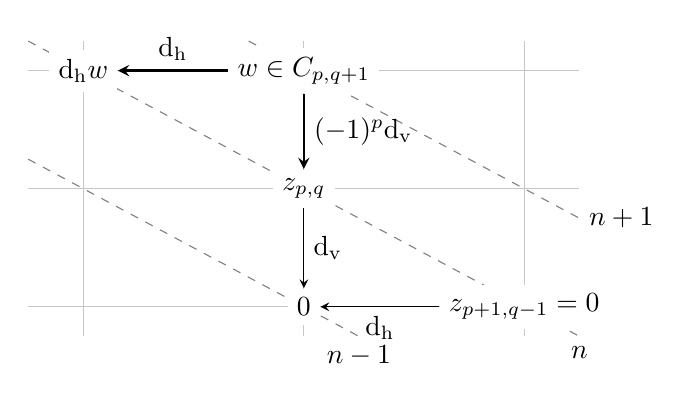
\begin{tikzpicture}[x=2.8cm,y=1.5cm,>=stealth]
\draw[gray!45,step=1] (-1.25,-1.25) grid (1.25,1.25);
\draw[dashed,gray] (-1.25,0.25)--(0.25,-1.25);
\draw[dashed,gray] (-1.25,1.25)--(1.25,-1.25);
\draw[dashed,gray] (-0.25,1.25)--(1.25,-0.25);
\node[fill=white] (w) at (0,1) {\(w\in C_{p,q+1}\)};
\node[fill=white] (z) at (0,0) {\(z_{p,q}\)};
\node[fill=white] (h) at (-1,1) {\(\mathrm d_{\mathrm h}w\)};
\node[fill=white] (v) at (0,-1) {\(0\)};
\node[fill=white] (r) at (1,-1) {\(z_{p+1,q-1}=0\)};
\draw[->,thick] (w)--(z) node[midway,right] {\((-1)^p\mathrm d_{\mathrm v}\)};
\draw[->,thick] (w)--(h) node[midway,above] {\(\mathrm d_{\mathrm h}\)};
\draw[->] (z)--(v) node[midway,right] {\(\mathrm d_{\mathrm v}\)};
\draw[->] (r)--(v) node[midway,below] {\(\mathrm d_{\mathrm h}\)};
\node[below] at (0.25,-1.25) {\(n-1\)};
\node[below] at (1.25,-1.25) {\(n\)};
\node[right] at (1.25,-0.25) {\(n+1\)};
\end{tikzpicture}
\end{center}
图中右侧分量为零，表示刚才选取最大横指标所排除的贡献。减去 \(\mathrm dw\) 消去 \(z_{p,q}\)，只在 \(C_{p-1,q+1}\) 留下修正 \(-\mathrm d_{\mathrm h}w\)，不会产生更右的分量。

于是 \(z-\mathrm{d}w\) 仍为圈，横指标 \(p\) 的分量已经消失，而新产生的分量至多位于横指标 \(p-1\)。第一象限中横指标不小于零，且次数 \(n\) 上只有 \(0\le p\le n\) 的位置；不断降低最大横指标，有限步后得到零。因此原圈是这些 \(w\) 的和的边界。横行正合时，交换两个指标；在 \(C_{p,q}\) 上乘符号 \((-1)^{pq}\)，给出交换前后两个全复形的同构，于是归入刚才的情形。
\end{proof}

\begin{lemma}[Tor 的平衡计算]\label{b3:lem:tor-balanced-computation}
设 \(R\) 为交换环，\(P_\bullet\rightarrow N\rightarrow0\) 与 \(Q_\bullet\rightarrow M\rightarrow0\) 为 \(R\) 模的自由消解。对每个整数 \(i\ge0\)，两条增广映射诱导自然同构
\[
H_i(P\otimes_RM)
\xleftarrow{\ \sim\ }H_i(\operatorname{Tot}(P\otimes_RQ))
\xrightarrow{\ \sim\ }H_i(N\otimes_RQ).
\]
因而用任一变量的自由消解都可计算 Tor，并有自然同构
\[
\operatorname{Tor}_i^R(N,M)\cong\operatorname{Tor}_i^R(M,N).
\]
\end{lemma}
\begin{proof}
取 \(C_{p,q}=P_p\otimes_RQ_q\)，水平、竖直微分分别为 \(\mathrm{d}_P\otimes1\)、\(1\otimes\mathrm{d}_Q\)。在纯张量上，全微分为
\[
\mathrm{d}(u\otimes v)=\mathrm{d}_Pu\otimes v+(-1)^p u\otimes\mathrm{d}_Qv.
\]
由 \(Q_0\twoheadrightarrow M\) 得到逐项满射
\(\alpha:\operatorname{Tot}(C)\rightarrow P\otimes_RM\)：它在 \(q=0\) 的分量上为增广映射，在 \(q>0\) 的分量上为零。这个映射把每条竖直消解在底端压到 \(P_p\otimes_RM\)。要保留被它删去的部分，核在 \(q>0\) 的位置仍取全部分量，底行则必须换成增广映射的核，而不能仍取整个 \(P_p\otimes_RQ_0\)。因此核是下面双复形 \(D\) 的全复形：
\[
D_{p,q}=P_p\otimes_RQ_q\quad(q>0),
\qquad
D_{p,0}=\ker(P_p\otimes_RQ_0\longrightarrow P_p\otimes_RM).
\]
水平微分与增广映射交换，所以保持底行的核；竖直微分从 \(q=1\) 出发时也落入这个核，故 \(D\) 确实是双复形。因为 \(P_p\) 自由，\(Q\) 的增广正合列张量 \(P_p\) 后仍正合，特别地从 \(P_p\otimes_RQ_1\) 到该底行核的映射满射。因此 \(D\) 的每条竖列正合，\cref{b3:lem:first-quadrant-column-exact}说明 \(\ker\alpha=\operatorname{Tot}(D)\) 正合。

这使 \(\alpha\) 在同调上成为同构：给 \(P\otimes_RM\) 中的圈任取提升，其微分落在核中；利用核的正合性减去适当核元素，便得到圈的提升。若全复形中的圈映为边界，先提升产生该边界的元素并减去它的微分，余下的圈落在核中，又是核中的边界。这分别证明满射与单射。

用 \(P_0\twoheadrightarrow N\) 得到另一条逐项满射
\(\beta:\operatorname{Tot}(C)\rightarrow N\otimes_RQ\)。此时将最左列 \(P_0\otimes_RQ_q\) 换成它到 \(N\otimes_RQ_q\) 的核，正是同样的截取。因每个 \(Q_q\) 自由，其核的每条横行正合，同一引理证明 \(\beta\) 也诱导同调同构。这就得到平衡计算。交换张量因子的映射
\[
u\otimes v\longmapsto(-1)^{pq}v\otimes u
\qquad(u\in P_p,\ v\in Q_q)
\]
保持全微分，并交换两条增广映射；于是得到 Tor 的对称性。对 \(N,M\) 的同态选比较链映射后，这些张量映射与增广映射交换；结合\cref{b3:cor:tor-well-defined-functor}的选择无关性，所述同构对两个变量都是自然的。因此以后选取较易消解的变量，并不会改变 Tor 模及其上由同态诱导的映射。
\end{proof}

\subsection{长正合列与 Koszul 计算}
\label{b3:subsec:1505:04}

\begin{lemma}\label{b3:lem:tor-basic-properties}
设 \(R\) 为交换环，\(N,M\) 为 \(R\) 模。Tor 具有自然同构
\[
\operatorname{Tor}_i^R(N,M)\cong\operatorname{Tor}_i^R(M,N)
\qquad(i\ge0),
\]
并在任一变量的短正合列上给出自然长正合列。例如，对 \(R\) 模短正合列
\(0\rightarrow M'\rightarrow M\rightarrow M''\rightarrow0\)，对整数 \(i\ge1\) 有
\[
\begin{aligned}
\cdots&\longrightarrow\operatorname{Tor}_i^R(N,M')
\longrightarrow\operatorname{Tor}_i^R(N,M)
\longrightarrow\operatorname{Tor}_i^R(N,M'')\\
&\xrightarrow{\delta}\operatorname{Tor}_{i-1}^R(N,M')
\longrightarrow\cdots\longrightarrow\operatorname{Tor}_1^R(N,M'')\\
&\xrightarrow{\delta}N\otimes_RM'
\longrightarrow N\otimes_RM
\longrightarrow N\otimes_RM''\longrightarrow0.
\end{aligned}
\]
若 \(a\in R\) 满足 \(aN=0\) 或 \(aM=0\)，则 \(a\operatorname{Tor}_i^R(N,M)=0\) 对每个 \(i\ge0\) 成立。若其中一个模平坦，则所有 \(i>0\) 的 Tor 为零。

对固定的 \(R\) 模 \(M\)，还有等价关系
\[
\begin{aligned}
M\;\text{平坦}
&\iff \operatorname{Tor}_1^R(N,M)=0
   \quad\text{对每个}\;R\;\text{模}\;N\\
&\iff \operatorname{Tor}_1^R(R/I,M)=0
   \quad\text{对每个理想}\;I\subseteq R.
\end{aligned}
\]
对任意理想 \(I,J\subseteq R\)，有自然同构
\[
\operatorname{Tor}_1^R(R/I,R/J)\cong(I\cap J)/IJ.
\]
\end{lemma}
\begin{proof}
对称性已由\cref{b3:lem:tor-balanced-computation}证明。固定 \(N\) 的自由消解 \(P\)，其各项自由，故给定短正合列张量 \(P_i\) 后仍正合，得到复形的逐项短正合列
\[
0\longrightarrow C'\xrightarrow{j}C\xrightarrow{q}C''\longrightarrow0,
\qquad
C'=P\otimes_RM',\quad C=P\otimes_RM,\quad C''=P\otimes_RM''.
\]
商复形中的圈任取一个提升后未必还是圈，但其微分误差必落在子复形中，并给出低一阶的圈；连接映射记录的就是这个误差的同调类。具体地，对 \(C''_i\) 中的圈 \(z''\)，取 \(C_i\) 中的提升 \(z\)。因 \(q(\mathrm{d}z)=0\)，存在唯一 \(z'\in C'_{i-1}\) 使 \(jz'=\mathrm{d}z\)。又由 \(j\) 单射及 \(j\mathrm{d}z'=\mathrm{d}^2z=0\)，有 \(\mathrm{d}z'=0\)。规定 \(\delta[z'']=[z']\)。改变提升只使 \(z'\) 增加一个边界；若 \(z''\) 增加边界 \(\mathrm{d}w''\)，提升 \(w''\) 并将其微分加到 \(z\) 上，\(z'\) 不变。因此连接映射良定义。

正合性在三类位置上直接核验。若 \(C\) 中的圈投到 \(C''\) 的边界，提升产生该边界的元素并减去其微分，便得到来自 \(C'\) 的圈。若 \(\delta[z'']=0\)，写 \(z'=\mathrm{d}v'\)，则 \(z-jv'\) 是 \(z''\) 的圈提升。若 \(C'\) 中的圈 \(z'\) 在 \(C\) 中成为边界 \(jz'=\mathrm{d}w\)，则 \(qw\) 为圈，且 \(\delta[qw]=[z']\)。这证明长列中各处正合；次数零的识别由\cref{b3:cor:tor-well-defined-functor}给出，末尾的满射由张量积右正合性得到。特别地，最低一段中 \(\delta\) 的像正是 \(N\otimes_RM'\to N\otimes_RM\) 的核，补回了张量后可能失去的单射信息。圈提升的构造与复形映射相容，故长列自然。第一变量的短正合列由平衡性得到相同结论。

若 \(aN=0\)，则 \(P\) 上的乘法 \(a\) 与零链映射都提升 \(N\) 上的零同态。\cref{b3:lem:free-resolution-comparison}给出它们之间的链同伦，张量 \(M\) 后仍成立，所以乘法 \(a\) 在同调上为零。若 \(aM=0\)，乘法 \(a\) 在 \(P\otimes_RM\) 上已为零。

若 \(M\) 平坦，令 \(Z_{-1}=N\)、\(Z_i=\ker\mathrm{d}_i\) 对 \(i\ge1\)，并令 \(Z_0=\ker(P_0\rightarrow N)\)。自由消解的正合性给出
\[
0\longrightarrow Z_i\longrightarrow P_i\longrightarrow Z_{i-1}\longrightarrow0
\qquad(i\ge0).
\]
每条短列张量 \(M\) 后仍正合，所以 \(P\otimes_RM\) 的正次数同调为零。若 \(N\) 平坦，交换两个变量即可。

反过来，若 \(\operatorname{Tor}_1^R(N,M)=0\) 对每个 \(N\) 成立，对任意短正合列 \(0\to U\to V\to W\to0\) 在第一变量中使用刚证的长列。\(\operatorname{Tor}_1^R(W,M)=0\) 使 \(U\otimes_RM\to V\otimes_RM\) 的核为零，故 \(M\) 平坦。更少的测试对象已经足够：对任意理想 \(I\)，因 \(R\) 自由，由 \(0\to I\to R\to R/I\to0\) 得到
\[
0\longrightarrow\operatorname{Tor}_1^R(R/I,M)
\longrightarrow I\otimes_RM\longrightarrow M.
\]
这里最后一个映射是 \(a\otimes m\mapsto am\)，所以 \(\operatorname{Tor}_1^R(R/I,M)\) 自然识别为理想张量判据中的核。若这些 Tor 对所有 \(I\) 都为零，\cref{b3:thm:ideal-flatness-criterion}便给出平坦性；前面已经证明平坦性使全部正次 Tor 消失，这完成所述等价关系。

在同一短列中取 \(M=R/J\)。映射
\(I\otimes_R(R/J)\to I/JI\)、\(a\otimes\bar r\mapsto ra+JI\)，与 \(a+JI\mapsto a\otimes\bar1\) 互逆；后一个映射良定义，因为 \(j\in J\) 时有 \(ja\otimes\bar1=a\otimes\bar j=0\)。因而得到
\[
0\longrightarrow\operatorname{Tor}_1^R(R/I,R/J)
\longrightarrow I/JI\longrightarrow R/J,
\qquad a+JI\longmapsto a+J.
\]
最后一个映射的核由恰好属于 \(J\) 的 \(a\in I\) 给出，即 \((I\cap J)/IJ\)。这证明交理想公式，且所有映射都来自包含、取商和张量积，因而同构自然。交 \(I\cap J\) 中未被乘积 \(IJ\) 消去的部分，由此成为一次 Tor 的具体表达。
\end{proof}

一般定义中的自由消解可以任意选择；当给定序列在 \(R\) 上正则时，前面构造的 Koszul 复形已经是 \(R/I\) 的自由消解，所以抽象的 Tor 可以直接用它的微分计算。

\begin{corollary}\label{b3:cor:koszul-tor}
设 \(R\) 为交换环，\(r\ge0\) 为整数，\(x=(x_1,\ldots,x_r)\) 是 \(R\) 上的正则序列，\(I=(x_1,\ldots,x_r)\)。对任意 \(R\) 模 \(M\) 与整数 \(i\ge0\)，有
\[
\operatorname{Tor}_i^R(R/I,M)\cong H_i(x;M).
\]
若 \(IM=0\)，则 \(\operatorname{Tor}_i^R(R/I,M)\cong M^{\binom ri}\) 对 \(0\le i\le r\) 成立，\(i>r\) 时为零。

特别地，设 \(k\) 为域，\(d\ge0\) 为整数，令
\[
R=k[X_1,\ldots,X_d]_{(X_1,\ldots,X_d)},
\qquad \mathfrak m=(X_1,\ldots,X_d)R,
\]
其剩余域 \(R/\mathfrak m\) 自然识别为 \(k\)。则对 \(0\le i\le d\)，有
\[
\operatorname{Tor}_i^R(k,k)\cong\bigwedge_k^ik^d,
\qquad
\dim_k\operatorname{Tor}_i^R(k,k)=\binom di;
\]
对 \(i>d\)，有 \(\operatorname{Tor}_i^R(k,k)=0\)。
\end{corollary}
\begin{proof}
用\cref{b3:thm:koszul-regular-resolution}给出的自由消解计算 Tor。若 \(IM=0\)，张量后的每个微分项 \(x_jm\) 都为零，同调就是复形本身各项，即所述的有限直和。

在局部多项式模型中，模掉 \(X_1,\ldots,X_{j-1}\) 后得到整环
\(k[X_j,\ldots,X_d]_{(X_j,\ldots,X_d)}\)，其中 \(X_j\) 非零，所以乘 \(X_j\) 单射。最终商为非零域 \(k\)，故变量序列是 \(R\) 正则序列；\(d=0\) 时则是空序列。其 Koszul 自由消解张量 \(k\) 后，所有 \(X_j\) 都作用为零，于是微分全为零，第 \(i\) 项按递增指标楔积基识别为 \(\bigwedge_k^ik^d\)。这组基的数目为 \(\binom di\)，且次数超过 \(d\) 时复形本身已经为零，得到所述同调与维数。
\end{proof}

在这个局部多项式模型中，\(k^d\) 通过标准基送到 \(X_j+\mathfrak m^2\)，识别为余切空间 \(\mathfrak m/\mathfrak m^2\)。因此一次 Tor 保留这些一次函数类，高次 Tor 则给出它们的外幂；由\cref{b3:prop:tangent-cotangent-rational}，切空间是这个余切空间的 \(k\) 线性对偶。
